% Seccion "Method" del paper de bin packing 3D (BSG_BPP).
% Requiere en el preambulo de main.tex (ademas de los paquetes actuales):
%   \usepackage{amssymb,amsthm,tikz}
%   \usetikzlibrary{arrows.meta,fit,backgrounds}
%   \newtheorem{proposition}{Proposition}
% Nombres de las configuraciones (F5, H20 y B100 en el README y en la bitacora)
\providecommand{\cfgfast}{\textsc{Fast}}
\providecommand{\cfgbal}{\textsc{Balanced}}
\providecommand{\cfgqual}{\textsc{Quality}}
\section{Method}
\label{sec:method}

The method treats bin packing as the generation and the recombination of bin patterns. A
pattern is the load of one bin, described by the number of boxes of each type that it contains.
In a first phase, a sequential construction heuristic is run many times while its priorities
are adjusted, and every bin that it produces is stored as a pattern. In a second phase, a set
covering or set partitioning model chooses, among the stored patterns, the combination that
loads all the boxes with the fewest bins: covering when removing a box from a bin keeps it
feasible, partitioning when it does not (for example, under vertical support). Figure~\ref{fig:overview} shows the pipeline.

The two phases are linked by a pool of patterns that is much larger than any solution that
contributes to it. One run of the construction yields as many patterns as bins, and the search
over priorities yields a new set of them at every iteration. Besides, each call to the bin
loader executes hundreds of complete greedy loads, and all of them are normally discarded except
the best; we keep the best few as additional patterns at almost no cost (Section~\ref{sec:m-pool}).
The set covering model can mix patterns that come from different iterations, which no single
iteration of the search can do, and the LP relaxation of the model indicates when the pool
contains nothing better than the incumbent solution.

\begin{figure}[t]
\centering
\begin{tikzpicture}[
  font=\footnotesize,
  box/.style={draw, rounded corners=2pt, align=center, minimum height=1.1cm, text width=2.5cm, fill=white, inner sep=3pt},
  pool/.style={box, fill=blue!8, draw=blue!60!black},
  box2/.style={box, minimum height=1.6cm},
  arr/.style={-{Stealth[length=5pt]}, thick},
  lab/.style={font=\scriptsize, fill=white, inner sep=1pt},
  phase/.style={draw=black!45, dashed, rounded corners=4pt, inner sep=8pt}
]
% Phase 1: search
\node[box]  (inst)   at (1.4,5.3)  {Instance\\ $d_t,\ v_t,\ (L,W,H)$};
\node[box]  (constr) at (7.0,5.3)  {Sequential construction\\ profits $p_t$};
\node[box]  (swo)    at (12.9,5.3) {Squeaky wheel\\ update weights $\omega_t$};
\node[box]  (bsg)    at (7.0,3.0)  {BSG loads one bin\\ ($\tau$ s per call)};
\node[pool] (pool)   at (1.4,3.0)  {Pattern pool $\mathcal{P}$\\ distinct bin loads};
\draw[arr] (inst) -- (constr);
\draw[arr] ([yshift=4pt]constr.east) -- node[lab,above]{solution $S$} ([yshift=4pt]swo.west);
\draw[arr] ([yshift=-4pt]swo.west) -- node[lab,below]{new $p_t$} ([yshift=-4pt]constr.east);
\draw[arr] ([xshift=-7pt]constr.south) -- node[lab,left]{boxes left} ([xshift=-7pt]bsg.north);
\draw[arr] ([xshift=7pt]bsg.north) -- node[lab,right]{bin} ([xshift=7pt]constr.south);
\draw[arr] (bsg.west) -- node[lab,above]{harvest} (pool.east);
\draw[arr] (constr.south west) -- node[lab,above,pos=0.45]{bins of $S$} (pool.north east);
% Phase 2: recombination
\node[box2] (lp)     at (1.4,-0.3)  {LP of the cover on $\mathcal{P}$\\ value $z$, duals $\lambda_t$};
\node[box2] (fix)    at (4.55,-0.3) {Reduced-cost fixing:\\ drop $r_j > |S^*|-1-z$};
\node[box2] (milp)   at (7.7,-0.3)  {MILP on the columns left\\ warm start $S^*$};
\node[box2] (rep)    at (10.85,-0.3){Repair: remove\\ surplus boxes};
\node[box2] (out)    at (14.0,-0.3) {Solution};
\draw[arr] (pool) -- (lp);
\draw[arr] (lp) -- (fix);
\draw[arr] (fix) -- (milp);
\draw[arr] (milp) -- (rep);
\draw[arr] (rep) -- (out);
\draw[arr] (rep.north) .. controls +(0,1.1) and +(0.7,1.1) .. ([xshift=0.7cm]lp.north)
  node[pos=0.5,lab,above]{repeat while it improves};
\node[lab,align=center,text width=2.5cm] (stop) at (1.4,-2.4) {stop if $\lceil z\rceil\ge|S^*|$:\\ $S^*$ is best in $\mathcal{P}$};
\draw[arr] (lp.south) -- (stop.north);
\begin{scope}[on background layer]
  \node[phase, fit=(inst)(constr)(swo)(bsg)(pool)] (ph1) {};
  \node[phase, fit=(lp)(fix)(milp)(rep)(out)(stop)] (ph2) {};
\end{scope}
\node[anchor=south west, font=\scriptsize\itshape] at (ph1.north west) {Phase 1: search, time limit $T$};
\node[anchor=north west, font=\scriptsize\itshape] at (ph2.south west) {Phase 2: recombination, time limit $T_{\mathrm{milp}}$};
\end{tikzpicture}
\caption{Overview of the method. The construction loads the bins one by one with BSG using the
profits $p_t$ of the box types; the squeaky wheel loop changes the profits from one construction
to the next. Every bin that BSG returns, and the best complete greedy loads that it explored
(harvest), are stored in the pool $\mathcal{P}$. The recombination phase solves the LP
relaxation of the set covering model over $\mathcal{P}$, removes the columns that cannot be in a
better solution and solves the remaining MILP, warm started with the best solution $S^*$.}
\label{fig:overview}
\end{figure}

\subsection{Notation}
\label{sec:m-notation}

The bins are identical, with dimensions $L\times W\times H$ and volume $V=LWH$. The $n$ boxes are
grouped into $m$ types of identical dimensions; type $t$ has volume $v_t$ and $d_t$ boxes, so
that $n=\sum_t d_t$. A \emph{load} is a set of boxes placed in a bin without overlaps, and its
\emph{pattern} is the vector $a\in\mathbb{Z}_{\ge 0}^{m}$ whose component $a_t$ is the number of
boxes of type $t$ in the load. A vector $a\le d$ is \emph{feasible} if there is a load with
pattern $a$. A solution $S$ is a list of loads whose patterns add up to $d$, and $|S|$ is the
number of bins. The search stops early when $|S|$ reaches the lower bound $\mathrm{LB}$ of
Section~\ref{sec:problem}.

\subsection{Loading one bin with BSG}
\label{sec:m-bsg}

Each bin is loaded by BSG, a beam search guided by a greedy algorithm \citep{Araya2014,Araya2017}
that places blocks of boxes in maximal free spaces. We summarise the elements that matter for
the rest of the method.

\paragraph{Blocks.}
A block is a cuboid arrangement of boxes that is placed as a unit. The blocks of one box are the
box in each allowed orientation, and further blocks are obtained by joining two blocks along the
$x$, $y$ or $z$ axis, as in \citet{Fanslau2010} and \citet{Araya2014}, so that every block has a
guillotine structure.
A joined block is kept if its boxes are still available, it fits in the bin, its boxes fill at
least a fraction $f_{\min}=0.98$ of its volume, and it differs from the blocks already generated.
The generation stops after $N_{\max}=500$ blocks.

\paragraph{Free spaces.}
The free volume of the bin is represented by the set of maximal free spaces \citep{Parreno2008}.
Every space is anchored at its corner closest to the origin of the bin, and the next space to be
filled is the one whose anchor is closest to the origin, with ties broken by larger volume. The
load therefore grows from one corner of the bin. An action places a block that fits in the
selected space at its anchor.

\paragraph{Evaluation of the blocks.}
The blocks that fit in the selected space are ranked with the VCS function of \citet{Araya2017},
in which the volume of the block is replaced by its profit:
\begin{equation}
\label{eq:vcs}
\mathrm{VCS}(b) = P(b)\,\bigl(1-\mathrm{loss}(b)\bigr)^{\beta}\,\mathrm{CS}_q(b)^{\alpha}\,|b|^{-\gamma}.
\end{equation}
Here $P(b)=\sum_t p_t\,\nu_t(b)$ is the profit of the block, where $\nu_t(b)$ is the number of boxes
of type $t$ in $b$ and $p_t$ is the profit of a box of type $t$ (Section~\ref{sec:m-construct});
$\mathrm{loss}(b)$ is the proportion of the free space that the remaining boxes cannot fill
after placing $b$, estimated with one-dimensional knapsack problems; $\mathrm{CS}_q(b)$ is the
proportion of the surface of $b$ in contact with placed blocks or walls, where a gap of at most
a proportion $q$ of the block dimension still counts as contact; and $|b|=\sum_t\nu_t(b)$ is the number of boxes
of $b$. We keep the values $\alpha=2.4407$, $\beta=2.2652$, $\gamma=0.3896$ and $q=0.0164$ that
were tuned for the container loading problem; we do not retune them for bin packing
(the sensitivity analysis is in Section~\ref{sec:e-ablation}).

\paragraph{Greedy and beam search.}
The greedy algorithm repeatedly selects the next free space and places in it the best ranked
block, until no block fits. The value of a complete load is the total profit of its boxes. BSG is
a beam search whose children are generated with the best ranked blocks for the selected space,
and each child is evaluated by the value of its greedy completion. The $B$ best children are kept
at each level, and the best complete load found by any greedy completion is returned. BSG is run
repeatedly with increasing effort until a time limit is reached \citep{Araya2017}: it starts with
$B=4$ and at most $C=16$ children per level, and after every run $B$ and $C/B$ are multiplied by
$\sqrt{2}$. The implementation applies the optimisations of \citet{Guesser2026}, which do not
change the result of the search.

In what follows, $\textsc{LoadBin}(R,p,\tau)$ denotes one such search of $\tau$ seconds over the multiset
of boxes $R$ with box profits $p$. It returns a load, its pattern $a\le R$, and the positions of
its boxes. The time $\tau$ covers the search and not the generation of the blocks, which costs a
fixed overhead of the order of two milliseconds per call. With very short limits BSG may end before completing
any greedy run; in that case one greedy run is completed without time limit, so that \textsc{LoadBin} always returns
a non-empty load when some box fits.

\subsection{Sequential construction with box profits}
\label{sec:m-construct}

The construction (Algorithm~\ref{alg:construct}) fills the bins one at a time. In each step
BSG loads a bin with the boxes that are still unplaced, and the boxes that it places are removed
from the instance. The loader is guided by profits instead of volumes. The profit of a box of
type $t$ is
\begin{equation}
\label{eq:profit}
p_t \;=\; V\left(\frac{v_t}{V}\right)^{\kappa},\qquad \kappa\ge 1 .
\end{equation}
With $\kappa=1$ the profit is the volume, and BSG maximises the filling of each bin. With
$\kappa>1$ a large box is worth more than its volume, so a bin that holds one more large box is
preferred to a bin with the same volume made of small boxes. Large boxes are thus loaded first
and the small ones, which fill the gaps best, remain for the bins that follow. We use $\kappa=2$ in all the experiments.

\begin{algorithm}[t]
\caption{$\textsc{Construct}(p)$}
\label{alg:construct}
\begin{algorithmic}[1]
\Require box profits $p$, demands $d$, time per bin $\tau$
\Ensure a solution $S$
\State $R\gets d$;\quad $S\gets\emptyset$
\While{$R\neq 0$}
  \State $(\ell,a)\gets \textsc{LoadBin}(R,p,\tau)$ \Comment{BSG, profit-guided}
  \State store $a$ in the pool $\mathcal{P}$ \Comment{with the positions of $\ell$}
  \State $R\gets R-a$;\quad append $\ell$ to $S$
\EndWhile
\State \Return $S$
\end{algorithmic}
\end{algorithm}

\subsection{Squeaky wheel optimisation of the box profits}
\label{sec:m-swo}

A single construction leaves a few bins with little load, usually the last ones, and which box
types end up there depends on the profits. Squeaky wheel optimisation \citep{Joslin1999} repeats
a construction, analyses the result, and raises the priority of the elements that were
troublesome. Here the elements are the box types, and the troublesome ones are those found in
the least loaded bins: they were hard to combine into well filled bins. Algorithm~\ref{alg:swo}
describes the loop.

Let $\omega_t$ be a weight of type $t$, initially one, so that the profit used in a construction is
$\omega_t\,p_t$ with $p_t$ from \eqref{eq:profit}. After each construction, the types that appear in
the $\max\{1,\mathrm{round}(0.1\,|S|)\}$ least loaded bins of that solution have their weight multiplied by
$1+\rho$, with $\rho=0.3$. Then every weight is multiplied by $e^{\varepsilon_t}$, where
$\varepsilon_t$ is drawn from a normal distribution with mean zero and standard deviation
$\sigma=0.05$. The weights accumulate along the iterations; they are neither reset nor decayed.
The noise breaks ties between types that are always treated alike and makes consecutive
constructions differ even when the set of troublesome types does not change.

The incumbent $S^*$ is replaced by a new solution when the latter has fewer bins or the same
number of bins and a smaller volume in its least loaded bin; the second criterion prefers
solutions that are closer to losing a bin. The loop ends when $|S^*|=\mathrm{LB}$ or when the
time limit $T$ is reached. The iteration in progress is completed, so the limit can be exceeded
by the duration of one construction.

\begin{algorithm}[t]
\caption{Squeaky wheel optimisation}
\label{alg:swo}
\begin{algorithmic}[1]
\Require instance, $\kappa$, $\rho$, $\sigma$, time limit $T$
\Ensure incumbent $S^*$ and pool $\mathcal{P}$
\State $\omega_t\gets 1$ for all $t$;\quad $S\gets \textsc{Construct}(p)$;\quad $S^*\gets S$
\While{$|S^*|>\mathrm{LB}$ \textbf{and} time $<T$}
  \State $M\gets$ the $\max\{1,\mathrm{round}(0.1\,|S|)\}$ least loaded bins of $S$
  \ForAll{types $t$}
    \If{some bin of $M$ contains a box of type $t$} $\omega_t\gets(1+\rho)\,\omega_t$ \EndIf
    \State $\omega_t\gets \omega_t\,e^{\varepsilon_t}$,\quad $\varepsilon_t\sim\mathcal{N}(0,\sigma^2)$
  \EndFor
  \State $S\gets \textsc{Construct}(\omega\cdot p)$
  \If{$S$ is better than $S^*$} $S^*\gets S$ \EndIf
\EndWhile
\State \Return $S^*$, $\mathcal{P}$
\end{algorithmic}
\end{algorithm}

\subsection{Pattern pool and harvest}
\label{sec:m-pool}

Every bin returned by \textsc{LoadBin} during the construction and the squeaky wheel loop is
stored in the pool $\mathcal{P}$. A pattern is stored once, whichever iteration produced it, and
the pool keeps the positions of the boxes of the first load found with that pattern. A pattern
in the pool is therefore always feasible, and a load is available for it.

\paragraph{Harvest.}
Each call to BSG executes many greedy completions, and each of them is a complete load of a bin,
but only the best one is returned. The harvest keeps some of the others. BSG notifies a callback
after every greedy completion. The callback computes the occupied volume $\upsilon$ of the
completed load and updates $\upsilon^*$, the largest volume seen in the current call. A load is
retained as a candidate if $\upsilon\ge\theta\,\upsilon^*$ and its pattern is neither in the pool
nor among the candidates. When the call ends, the candidates that still satisfy
$\upsilon\ge\theta\,\upsilon^*$ for the final value of $\upsilon^*$ are sorted by volume, and the
$K$ most loaded are added to the pool. To bound memory, when the candidates exceed $8K$ during the
call only the $K$ most loaded are kept. We use $K=10$ and $\theta=0.95$. The harvested loads are produced under the same state as
the load that BSG returns, with the same unplaced boxes, so they are valid columns for the covering
model, although the construction does not use them. The harvest acts whenever BSG loads an empty bin; it is not applied when BSG reloads a bin with
fixed boxes in the improvement phase of Appendix~\ref{app:improve}. The loads of the final solution are also added to the pool before the recombination.

The harvest does not alter any decision of BSG; it only records loads that BSG has already built,
at the cost of some extra time per call. Its effect is on the pool, which fills much faster per
second of search. This matters for short time limits, where the squeaky wheel loop alone would
produce too few patterns for the recombination to find a better combination
(Section~\ref{sec:e-ablation} isolates the effect of the harvest).

\subsection{Recombination by set covering or partitioning}
\label{sec:m-cover}

Let the columns $j\in\mathcal{P}$ be the patterns of the pool, with $a_{tj}$ boxes of type $t$ in
pattern $j$. The recombination solves
\begin{align}
\min\ & \sum_{j\in\mathcal{P}} x_j \label{eq:obj}\\
\text{s.t.}\ & \sum_{j\in\mathcal{P}} a_{tj}\,x_j \ge d_t \quad \forall t, \label{eq:cover}\\
& x_j\in\mathbb{Z}_{\ge 0}\quad\forall j, \label{eq:int}
\end{align}
where $x_j$ is the number of bins loaded with pattern $j$. The constraints are covering rather than
partitioning constraints: a combination of patterns may contain a box type more often than
demanded, and the surplus boxes are removed afterwards (see the repair step below). Variables are
general integers because the same pattern can be used in several bins. When removing a box can make
a load infeasible, as with vertical support (Section~\ref{sec:m-ext}), \eqref{eq:cover} is
replaced by the equalities $\sum_j a_{tj}x_j=d_t$ (\emph{partitioning model}); no box is then
removed and the repair step is not needed.

\paragraph{LP relaxation and pool bound.}
Let $z$ be the optimal value of the LP relaxation of \eqref{eq:obj}--\eqref{eq:int} and
$\lambda$ an optimal dual solution, with one price $\lambda_t$ per box type ($\lambda\ge 0$ in the
covering model, free in the partitioning model). The reduced
cost of column $j$ is
\begin{equation}
\label{eq:rc}
r_j \;=\; 1-\sum_t a_{tj}\,\lambda_t \;\ge\; 0 .
\end{equation}

\begin{proposition}
\label{prop:fix}
(i) Every solution of \eqref{eq:obj}--\eqref{eq:int} has at least $\lceil z\rceil$ bins.
(ii) If a solution has at most $U$ bins, then $x_j=0$ for every column $j$ with $r_j>U-z$.
\end{proposition}
\begin{proof}
Let $x$ be feasible. Using \eqref{eq:rc}, then $\lambda\ge 0$ together with \eqref{eq:cover}, and
finally strong duality ($z=\sum_t\lambda_t d_t$),
\[
\sum_j x_j=\sum_j r_j x_j+\sum_t\lambda_t\sum_j a_{tj}x_j\;\ge\;\sum_j r_j x_j+\sum_t\lambda_t d_t
\;=\;z+\sum_j r_j x_j .
\]
In the partitioning model the inequality is an equality and $\lambda\ge 0$ is not needed. Since
$r_j\ge 0$, $\sum_j x_j\ge z$, and the left side is an integer, which gives (i). If
$\sum_j x_j\le U$, the inequality gives $r_jx_j\le U-z$ for every $j$, so $x_j\ge 1$ requires
$r_j\le U-z$, which gives (ii).
\end{proof}

Part (ii) is reduced-cost fixing \citep{Wolsey1998}. The proposition is stated for the
columns of the pool. It says nothing about patterns that the pool does not contain, so $\lceil
z\rceil$ is a bound on what the pool can offer and not a lower bound on the optimum of the
instance.

\paragraph{Procedure.}
Algorithm~\ref{alg:recombine} starts from the incumbent $S^*$ of the search and looks for a
solution with at most $U=|S^*|-1$ bins. The patterns of $S^*$ are added to the pool, and the LP is
solved. If $\lceil z\rceil\ge|S^*|$, part (i) shows that the pool holds no better solution and
the procedure stops, which makes the MILP unnecessary
(Section~\ref{sec:e-recomb} reports in which fraction of the runs this happens). Otherwise, the
columns with $r_j>U-z$ are removed by part (ii) and the MILP is solved on the remaining columns
plus the columns of $S^*$, which are kept so that $S^*$ gives a feasible starting point for the
solver. The MILP returns an integer vector $x$, from which the repair step builds a solution. If
that solution has fewer bins than $S^*$, it becomes the new incumbent and the procedure starts
again with the new $U$; otherwise the procedure stops. The time limit $T_{\mathrm{milp}}$ is shared
by all the repetitions.

\paragraph{Repair.}
Given $x$, take $x_j$ copies of the load of every pattern $j$ with $x_j>0$. For each type $t$ with
a surplus $e_t=\sum_j a_{tj}x_j-d_t>0$, remove $e_t$ boxes of that type, taking them from the
copies that come last in a fixed order. The loads that become empty are discarded. A load that
loses a box remains feasible, because removing a box cannot create an overlap, so the result is a
valid solution with at most $\sum_j x_j$ bins. This holds only when no box needs another box below it;
with a vertical support requirement the removal could leave a box without support, and the
partitioning model is used instead (Section~\ref{sec:m-ext}).

\begin{algorithm}[t]
\caption{$\textsc{Recombine}(S^*,\mathcal{P},T_{\mathrm{milp}})$}
\label{alg:recombine}
\begin{algorithmic}[1]
\Require incumbent $S^*$, pool $\mathcal{P}$, time limit $T_{\mathrm{milp}}$
\Ensure a solution with $|S|\le|S^*|$
\State add the patterns of $S^*$ to $\mathcal{P}$;\quad $S\gets S^*$
\Loop
  \State solve the LP relaxation of \eqref{eq:obj}--\eqref{eq:int} on $\mathcal{P}$; get $z$ and $\lambda$
  \If{$\lceil z\rceil\ge|S|$} \State \Return $S$ \Comment{pool bound (i)}
  \EndIf
  \State $U\gets|S|-1$
  \State $\mathcal{P}'\gets\{j: r_j\le U-z\}\ \cup$ columns of $S$ \Comment{fixing (ii)}
  \State solve \eqref{eq:obj}--\eqref{eq:int} on $\mathcal{P}'$ with warm start $S$ within the time left; get $x$
  \State $S'\gets\textsc{Repair}(x)$
  \If{$|S'|<|S|$} $S\gets S'$ \Else \State \Return $S$ \EndIf
\EndLoop
\end{algorithmic}
\end{algorithm}

\begin{figure}[t]
\centering
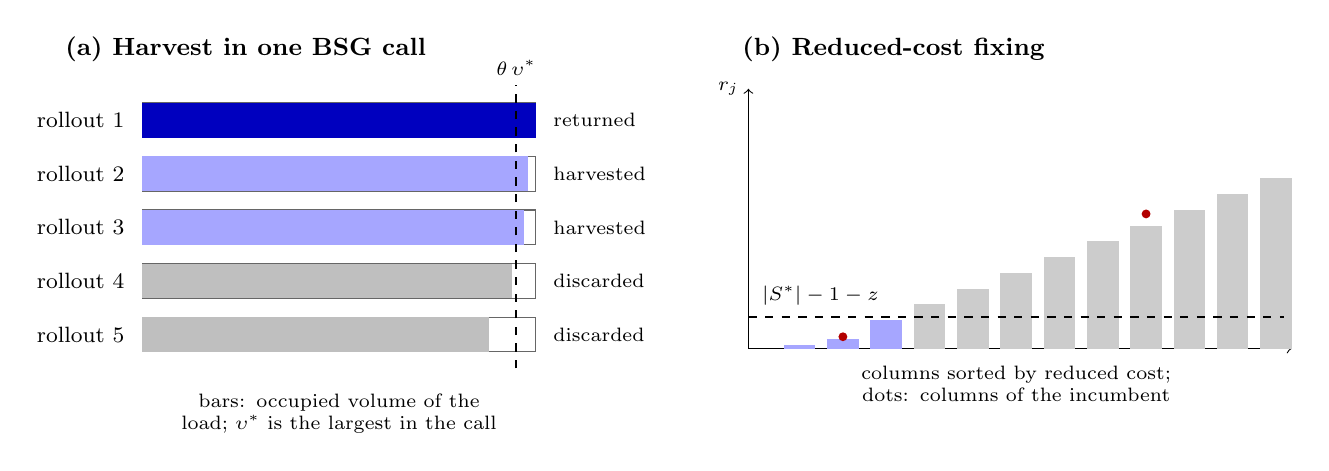
\begin{tikzpicture}[font=\footnotesize]
% (a) harvest in one BSG call
\node[font=\small\bfseries, anchor=west] at (0,4.2) {(a) Harvest in one BSG call};
\foreach \k/\vv/\col/\lbl in {0/100/blue!75!black/{returned},1/98/blue!35/{harvested},2/97/blue!35/{harvested},3/94/black!25/{discarded},4/88/black!25/{discarded}}{
  \pgfmathsetmacro{\yy}{3.3-0.68*\k}
  \node[anchor=east] at (1.0,\yy) {rollout \the\numexpr\k+1\relax};
  \draw[black!60] (1.1,\yy-0.22) rectangle (6.1,\yy+0.22);
  \pgfmathsetmacro{\bw}{1.1+5*\vv/100}
  \fill[\col] (1.1,\yy-0.22) rectangle (\bw,\yy+0.22);
  \node[anchor=west, font=\scriptsize] at (6.2,\yy) {\lbl};
}
\draw[dashed, thick] (5.85,0.15) -- (5.85,3.75);
\node[font=\scriptsize, anchor=south] at (5.85,3.75) {$\theta\,\upsilon^*$};
\node[font=\scriptsize, anchor=north, text width=6.2cm, align=center] at (3.6,-0.05) {bars: occupied volume of the load; $\upsilon^*$ is the largest in the call};
% (b) reduced-cost fixing
\node[font=\small\bfseries, anchor=west] at (8.6,4.2) {(b) Reduced-cost fixing};
\draw[->] (8.8,0.4) -- (8.8,3.7) node[left, font=\scriptsize] {$r_j$};
\draw[->] (8.8,0.4) -- (15.7,0.4);
\foreach \q/\rv in {1/0.1,2/0.3,3/0.9,4/1.4,5/1.9,6/2.4,7/2.9,8/3.4,9/3.9,10/4.4,11/4.9,12/5.4}{
  \pgfmathsetmacro{\xx}{8.9+0.55*\q}
  \pgfmathsetmacro{\hh}{0.4*\rv}
  \ifnum\q<4
    \fill[blue!35] (\xx-0.2,0.4) rectangle (\xx+0.2,0.4+\hh);
  \else
    \fill[black!20] (\xx-0.2,0.4) rectangle (\xx+0.2,0.4+\hh);
  \fi
}
\draw[dashed, thick] (8.8,0.8) -- (15.6,0.8);
\node[font=\scriptsize, anchor=south west] at (8.85,0.82) {$|S^*|-1-z$};
\fill[red!70!black] (8.9+0.55*2,0.55) circle (1.6pt);
\fill[red!70!black] (8.9+0.55*9,0.4+0.4*3.9+0.15) circle (1.6pt);
\node[font=\scriptsize, anchor=north, text width=7cm, align=center] at (12.2,0.3) {columns sorted by reduced cost; dots: columns of the incumbent};
\end{tikzpicture}
\caption{Schematic of two elements of the method (the values are illustrative). (a) One call to
BSG executes several greedy completions. The best one is returned to the construction, and the
others whose volume reaches $\theta\,\upsilon^*$ are added to the pool, up to $K$ of them. (b)
After the LP of the cover is solved, the columns whose reduced cost exceeds $|S^*|-1-z$ cannot be
in a solution with fewer bins than the incumbent and are removed (grey). The columns of the
incumbent stay in the model as the warm start, even when their reduced cost is above the threshold.}
\label{fig:harvest-fixing}
\end{figure}

\subsection{Overall algorithm}
\label{sec:m-overall}

Algorithm~\ref{alg:overall} puts the two phases together. Phase 1 spends the time limit $T$ on the
squeaky wheel loop, which builds the incumbent and fills the pool; Phase 2 spends at most
$T_{\mathrm{milp}}$ on the recombination. The time limits are independent, so the total running time
is about $T+T_{\mathrm{milp}}$, less when the lower bound is reached in Phase 1 or the pool bound
stops Phase 2. The result is checked box by box before it is reported.
The reduced costs used for the fixing are those that the LP solver returns at the optimum.

\begin{algorithm}[t]
\caption{Overall method}
\label{alg:overall}
\begin{algorithmic}[1]
\Require instance, $\kappa$, $\tau$, $K$, $T$, $T_{\mathrm{milp}}$
\Ensure a solution $S$
\State $(S^*,\mathcal{P})\gets$ squeaky wheel optimisation with time limit $T$ \Comment{Algorithm~\ref{alg:swo}, harvest with $K$}
\If{$T_{\mathrm{milp}}>0$ \textbf{and} $|S^*|>\mathrm{LB}$}
  \State $S\gets\textsc{Recombine}(S^*,\mathcal{P},T_{\mathrm{milp}})$ \Comment{Algorithm~\ref{alg:recombine}}
\Else
  \State $S\gets S^*$
\EndIf
\State check that $S$ is a valid packing of all the boxes
\State \Return $S$
\end{algorithmic}
\end{algorithm}

\subsection{Properties}
\label{sec:m-prop}

\paragraph{Validity and monotonicity.}
Every load that the method returns is a load that BSG built, possibly with some boxes removed
by the repair step, and the final check verifies box by box that the loads lie inside the bin, do
not intersect, and contain every box exactly once. The recombination starts from $S^*$, so it
never returns more bins than the search found.

\paragraph{What is guaranteed.}
When the LP bound stops the procedure, the incumbent is optimal \emph{for the pool}. The method
does not prove that it is optimal for the instance, and it does not search for patterns that are
not in the pool. Its quality depends on how well the construction and the harvest cover the
patterns that a good solution needs.

\paragraph{Cost.}
A construction needs one BSG call per bin, so it takes about $|S|\,(\tau+\delta)$ seconds, where
$\delta$ is the fixed overhead per call, and the squeaky wheel loop repeats it until the time
limit. The recombination adds the time of one LP and, when the LP bound does not stop it, of the
MILP, both bounded by $T_{\mathrm{milp}}$; HiGHS \citep{Huangfu2018} runs on a single thread.
The harvest adds the cost of one comparison of patterns per greedy completion.

\paragraph{Early stop by the pool bound.}
The implementation has an option that solves the LP of the pool every two seconds during the
squeaky wheel loop, once the first six seconds have passed. When $\lceil z\rceil\ge|S^*|$ it stops
the loop after $z$ has not decreased by more than $0.01$ in six seconds, so that $T$ becomes a
maximum, and when $\lceil z\rceil<|S^*|$ it tries the recombination at that point. We do not use the option in
the experiments of this paper, because the comparisons keep the time limits fixed.

\subsection{Rotations and vertical support}
\label{sec:m-ext}

\paragraph{Rotations.}
With rotations allowed, the generation of blocks includes the six orientations of every box. This
is the only change: the construction, the squeaky wheel loop, the pool and the recombination do
not depend on the orientation, because a pattern only counts boxes per type. The lower bound
used to stop the search is the continuous bound.

\paragraph{Vertical support.}
With the support requirement of Section~\ref{sec:problem}, only BSG and the recombination change.
Inside a block, one sub-block is stacked on another only if the lower one has a flat top that
covers the whole base of the upper one. A block placed above the floor is accepted only if every
box of its bottom layer has at least a fraction $0.7$ of its base area resting directly on the top
faces of the boxes below. The check is made when a block is placed, so every load that BSG returns,
and every harvested load, satisfies it. The recombination uses the partitioning model, so that no
box is removed from a load. The rest of the method is unchanged.
We tested the whole pipeline (squeaky wheel loop, harvest and partitioning recombination) on the industrial instances. The recombination did not improve any run there, and the construction alone with $\tau=2$ s and $\kappa=1$
is the better configuration for the large instances, and the loop alone for the small ones (Section~\ref{sec:e-ind}).

\subsection{Parameters and configurations}
\label{sec:m-params}

Table~\ref{tab:params} lists the parameters of the method, and Table~\ref{tab:configs} the three
configurations used in the experiments. They differ in the time limits of the search and of the
recombination, in the time per bin, and in whether the harvest is active. For a short search the
harvest compensates for the small number of squeaky wheel iterations; for a long search the
pool already holds many patterns without it.
With three seeds, \cfgqual{} with the harvest gives $7250.0\pm 1.0$ against $7249.3\pm 1.2$ without it ($p=0.72$), which supports leaving it out (Section~\ref{sec:e-mpv}).
The values of $\kappa$, $\rho$, $\sigma$, $\theta$ and $K$ were chosen on the original instances, and the sensitivity to $\rho$, $\sigma$, the fraction of least loaded bins, $K$, $\theta$ and $\tau$ is reported in Section~\ref{sec:e-ablation}.
\pend{Decide whether the noise $\sigma$ and the harvest threshold $\theta$ stay in the method. In the sensitivity analysis
(72 original instances, \cfgfast{}) $\sigma=0$ and $\theta=0.8$ were not worse than the defaults ($-2.0$ bins each, not
significant), so both could be removed (no noise; harvest the $K$ most loaded distinct loads without threshold). Confirm
with $\sigma=0$ and with $\theta=0$ on the 240 original instances and on the blind set before removing them.}
The method is implemented in C++ on top of the
Metasolver framework, with HiGHS 1.15.1 as the LP and MILP solver; the recombination is
compiled only when HiGHS is available. The implementation is available at \url{https://github.com/NicoFuentese/Metasolver} (branch \texttt{nico/bpp-mejoras}).

\begin{table}[t]
\centering
\caption{Parameters introduced by the method and the values used in all the experiments; the harvest size $K$ and the
time limits are part of the configurations (Table~\ref{tab:configs}). The parameters of BSG keep the values tuned for the
container loading problem \citep{Araya2017} and are given in Section~\ref{sec:m-bsg}; the minimum support of 70\% is part
of the problem (Section~\ref{sec:problem}).}
\label{tab:params}
\begin{tabular}{@{}llr@{}}
\toprule
Parameter & Symbol & Value\\
\midrule
Profit exponent & $\kappa$ & $2$\\
Weight increase of the types in the least loaded bins & $\rho$ & $0.3$\\
Standard deviation of the log-normal noise & $\sigma$ & $0.05$\\
Fraction of least loaded bins analysed & & $0.1$\\
Harvest threshold & $\theta$ & $0.95$\\
\bottomrule
\end{tabular}
\end{table}

\begin{table}[t]
\centering
\caption{Configurations. $T$: time limit of the squeaky wheel loop; $\tau$: BSG time per bin;
$K$: bins harvested per BSG call; $T_{\mathrm{milp}}$: time limit of the recombination, which adds to $T$.}
\label{tab:configs}
\begin{tabular}{@{}lrrrr@{}}
\toprule
Configuration & $T$ (s) & $\tau$ (s) & $K$ & $T_{\mathrm{milp}}$ (s)\\
\midrule
\cfgfast{}   & 4   & 0.005 & 10 & 30\\
\cfgbal{}  & 20  & 0.005 & 10 & 60\\
\cfgqual{} & 100 & 0.02  & 0  & 100\\
\bottomrule
\end{tabular}
\end{table}
